\chapter{Finetuning method to increase quality of document
embeddings}\label{chapter:training_method}

% \begin{itemize}

%     \item what this chapter is about

%     \item the contents of this chapter

%         \begin{itemize}

%             \item base model -

%             \item depth/breadth loss -- because it is complex we dedicate one section to each loss

%         \end{itemize}

% \end{itemize}

In this chapter we describe our finetuning method in detail. As we hinted at the
end of Chapter~\ref{chapter:document_representation} our finetuning method is
based on teacher-student training approach, where we distil the knowledge of
several teacher models into a single student model. First we present the idea
behind the training. Then we describe the teacher models in detail. Finally we
go over all components of our training loss in separate sections and define each
in concrete terms.

\section{Training methodology}

% \begin{itemize}
%     \item what is teacher-student training
%     \item our approach to training is to use teacher-student training
%     \item motivation to do so -- reference document representation chapter
%     \item two teachers -- depth and breadth teacher
% \end{itemize}

Our training methodology is based on how we evaluate a text embedding. As we
described in Chapter~\ref{chapter:document_representation} we view the quality
of text embeddings in two dimensions: depth and breadth. The depth dimension
defines how precise or detailed understanding of the text the embedding shows,
while the breadth dimension defines how much information the embedding is able
to reflect. We hypothesize that by increasing the amount of detail and of the
information that the embedding encodes, we improve the text embedding's
usefulness in the plethora of downstream tasks. We, therefore, aim to improve a
models' embeddings along each of the two dimensions. To do so we designed a
teacher-student training with two teachers, whose embeddings represent an ideal
in each of the two dimensions.

In the following subsections we describe teacher-student training in detail and
give high-level overview of the loss function we use.

\subsection{Teacher-student training}

In teacher-student training we train a single \emph{student} model according to
a non-trainable \emph{teacher} model. The idea is to make the student model to
imitate the teacher model and thereby digest the teacher's understanding of the
input. Typically there is an inherit limitation that prohibits straightforward
use of the teacher model and requires a model with different kind of qualities.
For instance \cite{sanh2019distilbert} used teacher-student training to reduce
the size of a model while retaining almost all of its performance. In another
experiment \cite{reimers2020making} overcame the insufficient training dataset
sizes to train an embedding model on low-resource languages.

In our setting we have two teacher models that correspond to the two aspects of
input understanding which we would like to instil to the student. We label the
teachers as depth teacher {\Md} and breadth teacher {\Mb}. We expect a
limitation of both of the teacher models that prevents their straightforward
use. As the depth teacher is oriented towards deep text understanding we expect
it will be unable to process longer inputs. On the other hand the breadth
teacher focuses on ingesting long texts and so we expect shallower understanding
of any given text sequence. Particularly for shorter inputs we expect {\Md} to
reflect their meaning better than {\Mb} and vice-versa for longer inputs.


\subsection{Abstract loss formulation}

% \begin{itemize}
%     \item there are two losses corresponding to the two reference models
%     \item weighting the two training losses -- depth model will not be applicable
%         for long inputs
% \end{itemize}

When computing the loss we take an embedding of each of the teacher model, and
of the student and define a loss based on their similarity. For each model we
have correspondingly labeled similarity-based losses. $\mathcal{L}_D$ compares
embedding of the student with that of the depth teacher {\Md} while
$\mathcal{L}_B$ with that of the breadth teacher {\Mb}. Let us also label the
input as $x$, the student's output as $y$, the depth teacher model's output as
$y_D$, and the breadth teacher model's output as $y_B$. Then the overall loss
has the following shape:

\begin{equation}
  \mathcal{L}(x, y, y_D, y_B, \lambda) =
    \lambda(x) \mathcal{L}_D(y, y_D) +
            \mathcal{L}_B(y, y_B),
\end{equation}

where $\lambda(x)$ is a weighting parameter that depends on the input $x$. This
is to reflect our expectation that for some inputs one loss reflects our goal
more than the other. For example shorter inputs it can be beneficial for
$\mathcal{L}_D$ to be dominant.

\subsection{Self-balancing out losses}

As we noted in earlier the two aspects of the embeddings, which we hope to
improve, stand in opposition. To illustrate this opposition on an example, let
us say we have a memory of limited size and a text. We can quite easily pack in
more detailed information about some of the words while forgetting the rest. We
can also forget all the minute little details about each word and make room to
remember few extra words. On the other hand doing both -- being more specific
about the words we already saved while making room to remember few extra ones --
seems like an impossible task. This balance between embedding's depth and
breadth is important to highlight because it plays role not only in the
performance of the final model but also during its training.

During evaluation some tasks may prefer the balance to be shifted one way or the
other. So it is crucial to choose tasks that reflect the diversity of text
embeddings' applications. During training the opposition between depth and
breadth plays to our advantage because optimizing one prohibits the model
overfitting on the other. For instance, we expect that if we leave out
$\mathcal{L}_B$ the student model would tend to forget the endings of longer
inputs. On the other hand by ignoring $\mathcal{L}_D$ the model could quickly
loose precision and many of the embeddings would become nearly identical.

\section{Reference models}

% \begin{itemize}
%     \item what models we used as teachers
%     \item why we chose as we did
% \end{itemize}

In this section we present the teacher models we later use during training. We
highlight how we obtain the teacher embeddings and what qualities we can expect
based on their previous evaluations and the models' architectures. We chose
Sentence-BERT~\cite{reimers2020making} (or SBERT) as the depth teacher model,
and Paragraph Vector~\cite{le2014distributed} (or PV) as the breadth teacher
model.

\subsection{SBERT}

Sentence-BERT~\cite{reimers2019sentence} is a composition of a
BERT-like~\cite{devlin2019bert} encoder with a mean pooling layer above its
final hidden states. While BERT-like architecture proved to be performant and
versatile useful not only for NLP (TODO:citation) SBERT focuses only on
generation of semantic embeddings of shorter text inputs.

The model is not trained from scratch. Instead it is warm started from a
checkpoint of BERT-like model such as RoBERTa~\cite{liu2019roberta} or
MPNet~\cite{song2020mpnet}. After adding a pooling layer the model is trained in
a siamese network structure, where two inputs are passed through the model after
which their embeddings are compared using a softmax classifier. SBERT is trained
on NLI datasets~\cite{bowman2015large},~\cite{williams2017broad} in which the
model is tasked to classify pairs of sentences as contradiction, entailment or
neutral.

To this day the authors provide a website\footnote{https://sbert.net} that
offers a selection of pre-trained SBERTs warm-started from different base
models. While each model has its advantages and shortcomings, we chose an SBERT
warm-started from MPNet, since it is reasonably small while providing the best
sentence embeddings according to the website's benchmarks. While the model's
maximum input length is only 384 tokens we believe that its performance
outweighs the shorter context, particularly given our training method.

We generate the embeddings of any training dataset directly without any
additional finetuning.

TODO: siamese networks schematic image here

\subsection{Paragraph Vector}

Paragraph Vector~\cite{le2014distributed} (also known as Doc2Vec) is a simple
text-embedding model that views the input as a Bag of Words (or BoW) (i.e. it
does not acknowledge word order). Architecturally it is an extension of
Word2Vec~\cite{mikolov2013efficient} which only embeds word.

Paragraph Vector is composed of two sub-models called Distributed Memory (or DM)
and Distributed Bag of Words (or DBOW). In practice one can use one or both
models and the final embedding is the concatenation of all used models. Both DM
and DBOW are trained on token prediction. To predict masked-out tokens, both
models use embedding of the whole input, while DM additionally computes word
embeddings. Embeddings of the whole input work as simply as any word embedding:
each piece of text (a word or an input) gets an identifier, which is associated
with a vector that is trained only for the given input. In practice this means
that PV must be trained on the dataset, whose embeddings it is supposed to
provide. Consequently there are no pretrained models and the prediction time is
rather long.

Though Paragraph Vector cannot match the performance of a substantially larger
models such as transformers, \cite{dai2015document} show that for larger
datasets it outperforms classical embedding models such as Latent Dirichlet
Allocation~\cite{blei2003latent} or TF-IDF weighted BoW
model~\cite{harris1954distributional}. Additionally its ability to embed
virtually limitlessly large sequences of text in combination with its small
size, is to this day unrivaled between embedding models.

We generate PV embeddings after training the model on \emph{all} datasets for
which we require a PV embedding. There are many hyperparameters that govern how
PV is trained such as the number of epochs, ignoring words based on frequency or
number of negative samples. Since there are no universally agreed
best-performing values for any of them, we see these as hyperparameters of our
teacher-student training method.

TODO: my own graphic here

\begin{figure}[h]
    \centering
    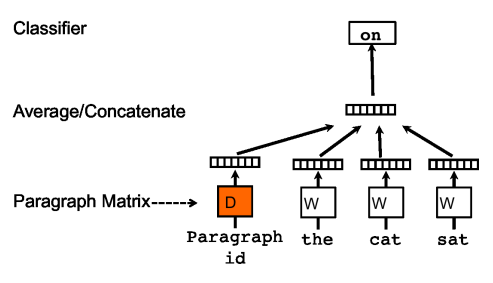
\includegraphics[width=0.4\textwidth]{./img/pv-dm.png}
    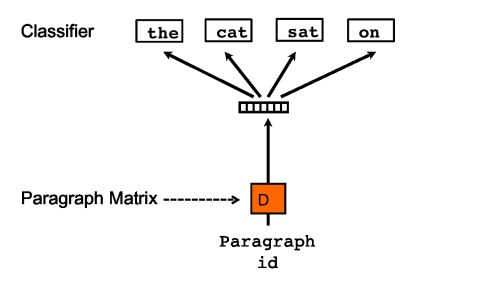
\includegraphics[width=0.4\textwidth]{./img/pv-dbow.png}
    \caption{PV-DM and PV-DBOW architectures.\label{fig:pv-dm_pv-dbow}}
\end{figure}

\section{Depth loss}

% \begin{itemize}
%     \item the depth loss is one of the two losses used
%     \item motivation for depth loss
% \end{itemize}

The depth loss $\mathcal{L}_D$ is one of the two losses our teacher-student
training will use. For inputs that fit into the maximum context length of the
depth teacher, the depth loss should minimize the dissimilarity between the
depth teacher's and the student's embeddings as much as possible. This follows
our assumption that for inputs that the depth model can process whole, the depth
model produces an embedding with the deepest understanding of the input that is
available to us. It is thus important that the similarity $\mathcal{L}_D$ should
take into account is the absolute similarity rather than some approximate
measure of it.

(TODO: What else to say about this? What dissimilarity we use will be in
Experiments chapter as well as deciding "when an input is applicable".)


\section{Breadth loss}

% \begin{itemize}
%     \item motivation for breadth loss
%     \item what should the loss do?
%     \item why should it do that
%     \item transition to CCA -- "this is exactly what CCA does, so we'll use it"
% \end{itemize}

The breadth loss $\mathcal{L}_B$ minimizes the disagreements between the
embeddings of the breadth teacher model {\Mb} and that of the student model.
There are two major differences between the breadth loss and the depth loss.
First the breadth loss is always applicable. It might not be the loss that
reflects our ultimate goal the most for the given input. Nevertheless we still
assume that for \emph{every} input the breadth teacher model offers some
information which the depth teacher model does not have. Second the breadth loss
is not as exact as the depth loss. Instead of forcing the teacher model to
adhere to two possibly very distinct ways how to encode information into a dense
vector representation, we give the model a little bit of freedom. We do so by
letting the model decide how exactly it should encode the information contained
in the breadth teacher's embedding. We give the model more leeway on the breadth
side rather than the depth side, because we expect that the precision of the
embedding is more important than capturing every piece of the input.

With the above taken into an account we chose to use a variant of
\emph{Canonical Correlation Analysis}~\cite{hotelling1992relations} (or
\emph{CCA}) as a base for our breath loss $\mathcal{L}_B$. A variant of CCA fits
our needs very nicely as it computes a correlation of outputs after some
projection. While the projection gives the model the freedom to restructure its
embeddings, the correlation ensures that the two embeddings agree with each
other. Before going further let us briefly describe CCA and its variants we
considered.

\subsection{Canonical Correlation Analysis}

Canonical Correlation Analysis (CCA) computes linear projections of two vectors
such that their projections are maximally correlated. For formal definition
reference Definition~\ref{def:cca}.

\begin{defn}[Canonical Correlation Analysis]\label{def:cca}

  For two matrices $X_1 \in \mathbb{R}^{n_1 \times m_1}$ and $X_2 \in
  \mathbb{R}^{n_2 \times m_1}$, Canonical Correlation Analysis finds $p \in
  \mathbb{R}^m_1$ and $q \in \mathbb{R}^m_2$ that maximize

  \begin{equation}
    \begin{split}
      & corr(X_1p, X_2q) = \frac{p^TX_1^TX_2q}{||Xp|| ||Yq||} \\
      \text{s.t.}\quad &||X_1p|| = ||X_2q|| = 1 \\
    \end{split}
  \end{equation}


\end{defn}

Definition~\ref{def:cca} suggests that CCA gives only a single number as the
measure of correlation of two matrices. When the dimensions of the input vectors
are large enough, however, often there exists at least one combination of
features that results in correlation of 1. As this would make CCA relatively
useless in the context of high-dimensional spaces we assume multiple
correlations for several mutually orthogonal projections. We name such Canonical
Correlation analysis as CCA for more dimensions and define it formally in
Definition~\ref{def:cca_more_dim}

\begin{defn}[Canonical Correlation Analysis for more dimensions]\label{def:cca_more_dim}

  For two matrices $X_1 \in \mathbb{R}^{n_1 \times m_1}$ and $X_2 \in
  \mathbb{R}^{n_2 \times m_1}$, Canonical Correlation Analysis for $k$
  dimensions finds $P \in \mathbb{R}^{m_1 \times k}$ and $Q \in \mathbb{R}^{m_2
  \times k}$ that maximize

  \begin{equation}
    \begin{split}
      &\sum_{i = 1}^k corr(X_1P_{*i}, X_2Q_{*i}) \\
      \text{s.t.}\quad &P^TX_1^TX_1P = I_k = Q^TX_2^TX_2Q \\
    \end{split}
  \end{equation}


\end{defn}

If we consider the conditions in Definition~\ref{def:cca_more_dim}, the
resulting value can be easily reformulated:

\begin{equation}
    \sum_{i = 1}^k corr(X_1P_{*i}, X_2Q_{*i}) =
    trace(P^TX_1^TX_2Q) =
    trace(P^T\Sigma_{X_1X_2}Q)
\end{equation}

Where $\Sigma_{X_1X_2}$ is the covariance matrix of $X_1$ and $X_2$.

TODO: analytical solution to pure CCA

\subsubsection{CCA as a breadth loss}

As we noted above we would like to use CCA as a base for our breadth loss
$\mathcal{L}_B$ in order to establish correspondence between the breadth
teacher's embedding and the student's. The problem using CCA as it was defined
in Definition~\ref{def:cca_more_dim} as a loss is that it is defined in the
context of the whole dataset rather than just a minibatch. It is therefore
unclear how should be CCA computed using just a pair of minibatches.

Someone (TODO: citation) found that using large enough batch size is sufficient
for the training to converge.

\subsubsection{Deep CCA}

Deep CCA (or DCCA) is an extension of CCA that computes projections using
neural networks. As such it is more powerful than plain CCA as it allows for
non-linear projections. To compute DCCA the network has to be trained on the
pairs of vectors with CCA as its loss.

TODO: graphic of architecture

If CCA is weaker condition than just correlation, DCCA is even weaker since
there is no limit to how the projections should look like.

\subsubsection{Soft CCA}

Soft CCA reformulates CCA and thus allows its straightforward use in the
context of minibatches. With constraints from Definition~\ref{def:cca_more_dim}
taken into account, CCA can be formulated using Forbenious matrix norm:

\begin{align}
  P^\ast, Q^\ast &= \underset{P, Q}{\argmin} ||X_1P - X_2Q||^2_F \\
  &= \underset{P, Q}{\argmin} trace\Big((X_1P - X_2Q)^T(X_1P - X_2Q)\Big) \\
  &= \underset{P, Q}{\argmin} {-2} trace(P^TX_1^TX_2Q) \\
  &= \underset{P, Q}{\argmax} trace(P^TX_1^TX_2Q) \\
  &= \underset{P, Q}{\argmax} \sum_{i = 1}^k corr(X_1P_{*i}, X_2Q_{*i})
\end{align}

So, in essence minimizing CCA is the same as minimizing the difference between
projections, whose features are decorrelated. This is the formulation Soft CCA
builds on. Soft CCA decomposes CCA into to parts:

\begin{itemize}
  \item minimization of the difference between projections

    \begin{equation}
      ||X_1P - X_2Q||^2_F
    \end{equation}

  \item decorrelation of each projection $P$

    \begin{equation}
      \sum_{i \ne j} (P^TX^T_{mini}X_{mini}P)_{ij} = \sum_{i \ne j} \Sigma_{X_{mini}P},
    \end{equation}

    where $X_{mini}$ is batch-normalized minibatch.

\end{itemize}

To bring correlation matrix of the current minibatch $\Sigma_{X_{mini}P}$
closer to the true covariance, the decorrelation part is in fact computed from
a covariance matrix that is incrementally learned.

In this way Soft CCA incrementally decreases CCA through incrementally learned
approximation of the projections' covariances.

\subsubsection{Loss selection}

\begin{itemize}
    \item mention which of the CCA variants we chose
    \item reiterate the formulation in the context of teacher-student training
\end{itemize}
